%Copyright 2017 R.D. Martin
%This book is free software: you can redistribute it and/or modify it under the terms of the GNU General Public License as published by the Free Software Foundation, either version 3 of the License, or (at your option) any later version.
%
%This book is distributed in the hope that it will be useful, but WITHOUT ANY WARRANTY; without even the implied warranty of MERCHANTABILITY or FITNESS FOR A PARTICULAR PURPOSE.  See the GNU General Public License for more details, http://www.gnu.org/licenses/.
\chapter{Describing motion in one dimension}
\label{Kinematics1D}
In this chapter, we will introduce the tools required to describe motion in one dimension. In later chapters, we will use the theories of physics to model the motion of objects, but first, we need to make sure that we have the tools to describe the motion. We generally use the word ``kinematics'' to label the tools for describing motion (e.g. speed, acceleration, position, etc), whereas we refer to ``dynamics'' when we use the laws of physics to predict motion (e.g. what motion will occur if a force is applied to an object). 
 \vspace{1cm}
\begin{openingSA}
You are taking your 6 year old cousin, Lily, to see the aquarium in Toronto. You are sitting on the train in Kingston waiting to leave the station. Lily exclaims that your train must be moving, and is excited that you are on your way to Toronto. You wonder why she said this, so you look out the window and notice that train beside you is moving backwards. You conclude that your train is not moving after all. How do you explain this to Lily? Do you know for certain that you aren't moving?
\end{openingSA}
\vspace{12pt}
\begin{learningObjectives}
\item Describe motion in 1D using functions and defining an axis.
\item Define position, velocity, speed, and acceleration.
\item Use calculus to describe motion.
\item Define the meaning of an inertial frame of reference.
\item Use Galilean and Lorentz transformations to convert the description of an object's position from one inertial frame to another.
\end{learningObjectives}


The most simple type of motion to describe is that of a particle that is constrained to move along a straight line (one-dimensional motion); much like a train along a straight piece of track. When we say that we want to describe the motion of the particle (or train), what we mean is that we want to be able to say where it is at what time. Formally, we want to know the particle's \textbf{position as a function of time}, which we will label as $x(t)$. The function will only be meaningful if:
\begin{itemize}
\item we specify an $x$-axis and the direction that corresponds to increasing values of $x$
\item we specify an origin where $x=0$
\item we specify the units for the quantity, $x$.
\end{itemize}
That is, unless all of these are specified, you would have a hard time describing the motion of an object to one of your friends over the phone. 

\capfig{0.4\textwidth}{figures/DescribingMotionIn1D/1daxis.png}{\label{fig:DescribingMotionIn1D:1daxis.png}In order to describe the motion of the grey ball along a straight line, we introduce the x-axis, represented by an arrow to indicate the direction of increasing $x$, and the location of the origin, where $x=\SI{0}{m}$. Given our choice of origin, the ball is currently at a position of $x=\SI{0.5}{m}$.
}
Consider Figure \ref{fig:DescribingMotionIn1D:1daxis.png} where we would like to describe the motion of the grey ball as it moves along a straight line. In order to quantify where the ball is, we introduce the ``$x$-axis'', illustrated by the black arrow. The direction of the arrow corresponds to the direction where $x$ increases (i.e. becomes more positive). We have also chosen a point where $x=0$, and by convention, we choose to express $x$ in units of meters (the S.I. unit for the dimension of length).

Note that we are completely free to choose both the direction of the $x$-axis and the location of the origin. The $x$-axis is a mathematical construct that we introduce in order to describe the physical world; we could just as easily have chosen for it to point in the opposite direction with a different origin. Since we are completely free to choose where we define the $x$-axis, we should choose the option that is most convenient to us. 

\section{Motion with constant speed}
Now suppose that the ball in Figure \ref{fig:DescribingMotionIn1D:1daxis.png} is rolling, and that we recorded its x position every second in a table and obtained the values in Table \ref{tab:DescribingMotionIn1D:1dmotion} (we will ignore measurement uncertainties and pretend that the values are exact).
\begin{table}[!h]
\centering
\begingroup
\renewcommand{\arraystretch}{1.0}
\begin{tabular}{cc}
\textbf{Time [s]}&\textbf{X position [m]}\\
\hline
\hline
\SI{0.0}{s}& \SI{0.5}{m}\\ \hline
\SI{1.0}{s}& \SI{1.0}{m}\\ \hline
\SI{2.0}{s}& \SI{1.5}{m}\\ \hline
\SI{3.0}{s}& \SI{2.0}{m}\\ \hline
\SI{4.0}{s}& \SI{2.5}{m}\\ \hline
\SI{5.0}{s}& \SI{3.0}{m}\\ \hline
\SI{6.0}{s}& \SI{3.5}{m}\\ \hline
\SI{7.0}{s}& \SI{4.0}{m}\\ \hline
\SI{8.0}{s}& \SI{4.5}{m}\\ \hline
\SI{9.0}{s}& \SI{5.0}{m}\\ \hline
\end{tabular}
\caption{\label{tab:DescribingMotionIn1D:1dmotion} Position of a ball along the x-axis recorded every second.}
\endgroup
\end{table}
The easiest way to visualize the values in the table is to plot them on a graph. Plotting position as a function of time is one of the most common graphs to make in physics, since it is often a complete description of the motion of an object. We can easily plot these values in Python:
\begin{python}[caption=Plotting position versus time] 
#First, we load pylab module for plotting
import pylab as pl
#We define t as a list of values (note the square brackets):
t = [0.0, 1.0, 2.0, 3.0, 4.0, 5.0, 6.0, 7.0, 8.0, 9.0]
#Similarly, we define the corresponding positions:
x = [0.5, 1.0, 1.5, 2.0, 2.5, 3.0, 3.5, 4.0, 4.5, 5.0]
#Define the plot:
pl.plot(t,x,'.')# the '.' means that it will show the actual points instead of a line
#Set the range of the axes, add some labels and a grid
pl.ylim(0,6)
pl.xlim(0,10)
pl.xlabel('time [s]')
pl.ylabel('position [m]')
pl.grid()
#Show the plot
pl.show()
\end{python}
\begin{poutput}
(* \capfig{0.7\textwidth}{figures/DescribingMotionIn1D/1dxvst.png}{\label{fig:DescribingMotionIn1D:1dxvst}Plot of position as a function of time using the values from Table \ref{tab:DescribingMotionIn1D:1dmotion}.} *)
\end{poutput}

The data plotted in Figure \ref{fig:DescribingMotionIn1D:1dxvst} show that the $x$ position of the ball increases linearly with time (i.e. it is a straight line). This means that in equal time increments, the ball will cover equal distances. Note that we also had the liberty to choose when we define $t=0$; in this case, we chose that time is zero when the ball is at $x=\SI{0.5}{m}$. 

\begin{checkpointSA}{Using the data from Table \ref{tab:DescribingMotionIn1D:1dmotion}, at what position along the x-axis will the ball be when time is $t=\SI{9.5}{s}$, if it continues its motion undisturbed?} %5.25m
\end{checkpointSA} 

Since the position as a function of time for the ball plotted in Figure \ref{fig:DescribingMotionIn1D:1dxvst} is linear, we can summarize our description of the motion using a function, $x(t)$, instead of having to tabulate the values as we did in Table \ref{tab:DescribingMotionIn1D:1dmotion}. The function will have the functional form:
\begin{align*}
x(t) = a + b t
\end{align*}
The constant $a$ is the ``offset'' of the function, the value that the function has at $t=\SI{0}{s}$. The constant $b$ is the slope and gives the rate of change of the position as a function of time. We can determine the values for the constants $a$ and $b$ by choosing any two rows from Table \ref{tab:DescribingMotionIn1D:1dmotion} (to determine 2 unknown quantities, you need 2 equations), and obtain 2 equations and 2 unknowns. For example, choosing the points where $t=\SI{0}{s}$ and $t=\SI{2.0}{s}$:
\begin{align*}
x(t=\SI{0}{s})&=\SI{0.5}{m}=a + b(\SI{0}{s}) \\
x(t=\SI{2.0}{s})&=\SI{1.5}{m}=a + b(\SI{2.0}{s}) \\
\end{align*}
The first equation immediately gives $a = \SI{0.5}{m}$, which we can substitute into the second equation to get $b$:
\begin{align*}
\SI{1.5}{m}&=a + b(\SI{2.0}{s}) = \SI{0.5}{m} + b(\SI{2.0}{s})\\
\therefore b &=\frac{(\SI{1.5}{m})-(\SI{0.5}{m})}{(\SI{2.0}{s})}=\SI{0.5}{m/s}
\end{align*}
which gives us the functional form for $x(t)$:
\begin{align*}
x(t) = (\SI{0.5}{m}) + (\SI{0.5}{m/s}) t
\end{align*}
where you should note that $a$ and $b$ have different dimensions. Since $a$ is added to something that must then give dimensions of length (for position, $x$), $a$ has dimensions of length. $b$ is multiplied by time, and that product must have dimensions of length as well; $b$ thus has dimensions of length over time, or ``speed'' (with S.I. units of \si{m/s}).

We can generalize the description of an object whose position increases linearly with time as:
\begin{align}
\label{eqn:DescribingMotionIn1D:1dxvst_noa}
\Aboxed{x(t) = x_0 + v_xt}
\end{align}
where $x_0$ is the position of the object at time $t=\SI{0}{s}$ ($a$ from above), and $v_x$ corresponds to the distance that the object covers per unit time ($b$ from above) along the x-axis. We call $v_x$ the ``velocity'' of the object. If $v_x$ is large, then the object covers more distance in a given time, i.e. it moves faster. If $v_x$ is a negative number, then the object moves in the negative $x$ direction.

\capfig{0.7\textwidth}{figures/DescribingMotionIn1D/1dturn.png}{\label{fig:DescribingMotionIn1D:1dturn}Position as a function of time for an object.}
\begin{checkpointMC}{Referring to Figure \ref{fig:DescribingMotionIn1D:1dturn}, what can you say about the motion of the object? }
\item The object moved faster and faster between $t=\SI{0}{s}$ and $t=\SI{30}{s}$, then slowed down to a stop at $t=\SI{60}{s}$.
\item The object moved in the positive x-direction between $t=\SI{0}{s}$ and $t=\SI{30}{s}$, and then turned around and moved in the negative x-direction between $t=\SI{30}{s}$ and $t=\SI{60}{s}$. %correct
\item The object moved faster between $t=\SI{0}{s}$ and $t=\SI{30}{s}$ than it did between $t=\SI{30}{s}$ and $t=\SI{60}{s}$.
\end{checkpointMC}

\capfig{0.7\textwidth}{figures/DescribingMotionIn1D/1d2objects.png}{\label{fig:DescribingMotionIn1D:1d2objects}Positions as a function of time for two objects.}
\begin{checkpointMC}{Referring to Figure \ref{fig:DescribingMotionIn1D:1d2objects}, what can you say about the motion of the two objects? }
\item Object 1 is slower than Object 2
\item Object 1 is more than twice as fast as Object 2 %correct
\item Object 1 is less than twice as fast as Object 2
\end{checkpointMC}

\section{Motion with constant acceleration}
Until now, we have considered motion where the velocity is a constant (i.e. where velocity does not change with time). Suppose that we wish to describe the position of a falling object that we released from rest at time $t=\SI{0}{s}$. The object will start with a velocity of \SI{0}{m/s} and it will \textbf{accelerate} as it falls. We say that an object is ``accelerating'' if its velocity is not constant. As we will see in later chapters, objects that fall near the surface of the Earth experience a constant acceleration (their velocity changes at a constant rate).

Formally, we define acceleration as the rate of change of velocity. Recall that velocity is the rate of change of position, so acceleration is to velocity what velocity is to position. In particular, we saw that if the velocity, $v_x$, is constant, then position as a function of time is given by:
\begin{align}
x(t) = x_0 + v_xt \tag{\ref{eqn:DescribingMotionIn1D:1dxvst_noa}}
\end{align} 
In analogy, if the acceleration is constant, then the velocity as a function of time is given by:
\begin{align}
\label{eqn:DescribingMotionIn1DL1dvvst}
\Aboxed{v_x(t) = v_{0x} + a_xt }
\end{align}
where $a_x$ is the ``acceleration'' and $v_{0x}$ is the velocity of the object at $t=0$. We can work out the dimensions of acceleration for this equation to make sense. Since we are adding $v_{0x}$ and $a_xt$, we need the dimensions of $a_xt$ to be velocity:
\begin{align*}
[a_xt] &= \frac{L}{T} \\
[a_x][t] &= \frac{L}{T} \\
[a_x]T&= \frac{L}{T} \\
[a_x]&= \frac{L}{T^2} \\
\end{align*}
Acceleration thus has dimensions of length over time squared, with corresponding S.I. units of m/s$^2$ (meters per second squared or meters per second per second). 

Now that we have an understanding of acceleration, how do we describe the position of an object that is accelerating? We cannot use equation \ref{eqn:DescribingMotionIn1D:1dxvst_noa}, since it is only correct if the velocity is constant. 

\capfig{0.1\textwidth}{figures/DescribingMotionIn1D/1daxis_vertical.png}{\label{fig:DescribingMotionIn1D:1daxis_vertical} X-axis for an object that starts at rest at $x=\SI{0}{m}$ when $t=\SI{0}{s}$ and falls downwards (in the direction of increasing $x$).}

Let us work out the corresponding equation for position as a function of time for accelerated motion using the x-axis depicted in Figure \ref{fig:DescribingMotionIn1D:1daxis_vertical}. We will determine $x(t)$ for the grey ball that starts at rest ($v_{0x}=\SI{0}{m/s}$) at the position $x=\SI{0}{m}$ at time $t=\SI{0}{s}$ with a constant positive acceleration $a_x=\SI{10}{m/s\squared}$. We would like to use equation \ref{eqn:DescribingMotionIn1D:1dxvst_noa}, but we cannot because it only applies if the velocity is constant. To remedy this, we pretend (we ``approximate'') that for a very small amount of time, the velocity is almost constant. Let us take a very small interval in time, say $\Delta t=\SI{0.001}{s}$, and approximate that the velocity is constant during that interval. 

At $t=\SI{0}{s}$, we have $x=\SI{0}{m}$, $v_{0x}=\SI{0}{m/s}$ and $a_x=\SI{10}{m/s\squared}$. We can use equation \ref{eqn:DescribingMotionIn1DL1dvvst} to find the velocity at $t=\Delta t$ (at the end of the first interval):
\begin{align*}
v_x(t=\Delta t) &= v_{0x} + a_x\Delta t\\
&=(\SI{0}{m/s})+ a_x\Delta t\\&=a_x\Delta t
\end{align*}

The average velocity during the first interval, $v_1^{avg}$ is then given by averaging the velocity at the beginning and at the end of the interval:
\begin{align*}
v_1^{avg}(t=\Delta t)&=\frac{1}{2}\left[ v(t=0) + v(t=\Delta t)\right]\\
&=\frac{1}{2}\left(v_{0x}+a_x\Delta t\right)\\
&=\frac{1}{2}\left((\SI{0}{m/s})+a_x\Delta t\right)\\
&=\frac{1}{2}(\SI{10}{m/s^2})(\SI{0.001}{s})\\
&=\SI{0.005}{m/s}
\end{align*}
Using the average velocity during the interval, we can use equation \ref{eqn:DescribingMotionIn1D:1dxvst_noa} to find the position at $t=\Delta t$: 
\begin{align*}
x(t=\Delta t) &= x_0 +v_1^{avg}\Delta t\\
&=(\SI{0}{m}) + \frac{1}{2}a_x(\Delta t)^2\\
&= \frac{1}{2}(\SI{10}{m/s^2})(\SI{0.001}{s})^2\\
&=\SI{0.000005}{m}
\end{align*}
Thus, at time $t=\SI{0.001}{s}$, the object will have a velocity of $v=\SI{0.005}{m/s}$ and be at a position $x=\SI{0.000005}{m}$. We can now use these values as the starting velocity and position for the next interval in time. Using variables, at the beginning of the second interval, the velocity is $v(t=\Delta t)=a_x\Delta t$ and at the end of the second interval, it will be $v(t=2\Delta t)=2a_x\Delta t$. The average velocity during the second interval is thus given by:
\begin{align*}
v_2^{avg}(t=2\Delta t)&= \frac{1}{2}\left[v(t=\Delta t)+v(t=2\Delta t) \right]\\
&=\frac{1}{2}(a_x\Delta t+2a_x\Delta t)\\
&=\frac{3}{2}a_x\Delta t\\
&=\frac{3}{2}(\SI{10}{m/s^2})(\SI{0.001}{s})\\
&=\SI{0.015}{m/s}
\end{align*}
To find the position at the end of the second time interval, when $t=2\Delta t$, we use equation \ref{eqn:DescribingMotionIn1D:1dxvst_noa} again, but with a different starting position and the average velocity that we just found:
\begin{align*}
x(t=2\Delta t) &= x(t=\Delta t) +v_2^{avg}\Delta t\\
&= \frac{1}{2}a_x(\Delta t)^2+\frac{3}{2}a(\Delta t)^2\\
&= \frac{1}{2}a_x(2\Delta t)^2\\
&=\frac{1}{2}(\SI{10}{m/s^2})(2\times\SI{0.001}{s})^2=\SI{0.00002}{m}
\end{align*}
You can carry out this exercise to ultimately find the position at any time. However, if you carry it out over a few more intervals, you may notice the following pattern: For the Nth interval when $t=N\Delta t$ at the end of the interval, we have:
\begin{align*}
v(t=(N-1)\Delta t) &= a_x (N-1) \Delta t &\text{(at beginning of interval N)}\\
v(t=N\Delta t) &= a_x N \Delta t &\text{(at end of interval N)}\\
v_N^{avg}&=\frac{1}{2}a_x(2N-1)\Delta t&\text{(average during interval)}\\
x(t=N\Delta t)&=\frac{1}{2}a_x(N\Delta t)^2&\text{(position at end of interval)}
\end{align*}

The last line gives us exactly what we were after, namely the position as a function of time for a constant acceleration, $a_x$, when the object started at rest at a position of $x=\SI{0}{m}$:
\begin{align}
\label{eqn:DescribingMotionIn1D:1dxoft_novonoxo}
 x(t) = \frac{1}{2} a_x t^2
\end{align}

If at $t=0$, the object had an initial position along the x-axis of $x_0$, then the position $x(t)$ would be shifted by an amount $x_0$:

\begin{align}
\label{eqn:DescribingMotionIn1D:1dxoft_novo}
 x(t) = x_0+\frac{1}{2} a_x t^2
\end{align}

Finally, if the object had an initial speed $v_{0x}$ at $t=0$, one can easily reproduce the iterations above to find that we need to add an additional term to account for this. We arrive at the general description of the position of an object moving in a straight line with acceleration, $a_x$:
\begin{align}
\label{eqn:DescribingMotionIn1D:1dxvst}
\Aboxed{ x(t) = x_0+v_{0x}t+ \frac{1}{2}a_xt^2}
\end{align}
Note that equation \ref{eqn:DescribingMotionIn1D:1dxvst_noa} is just a special case of the above when $a=0$. 

\begin{example}{A ball is thrown upwards with a velocity of \SI{10}{m/s}. After which distance will the ball stop before falling back down? Assume that gravity causes a constant downwards acceleration of \SI{9.8}{m/s^2}.}
\label{ex:DescribingMotionIn1D:ballupandown}
We will solve this problem in the following steps:
\begin{enumerate}[topsep=-10pt]
\item Setup a coordinate system (define the x-axis).
\item Identify the condition that corresponds to the ball stopping its upwards motion and falling back down.
\item Determine the distance at which the ball stopped.
\end{enumerate}
Since we throw the ball upwards with an initial velocity upwards, it makes sense to choose an x-axis that points up and has the origin at the point where we release the ball. With this choice, referring to the variables in equation \ref{eqn:DescribingMotionIn1D:1dxvst}, we have:
\begin{align*}
x_0&=0\\
v_{0x}&=+\SI{10}{m/s}\\
a_x&=\SI{-9.8}{m/s^2}
\end{align*}
where the initial velocity is in the positive x-direction, and the acceleration, $a_x$, is in the negative direction (the velocity will be getting smaller and smaller, so its rate of change is negative).

The condition for the ball to stop at the top of the trajectory is that its velocity will be zero (that is what it means to stop). We can use equation \ref{eqn:DescribingMotionIn1DL1dvvst} to find what time that corresponds to:
\begin{align*}
v(t) &= v_{0x}+a_xt\\
0 &= (\SI{10}{m/s}) + (\SI{-9.8}{m/s^2})t\\
\therefore t&=\frac{(\SI{10}{m/s})}{(\SI{9.8}{m/s^2})}=\SI{1.02}{s}
\end{align*}
Now that we know that it took \SI{1.02}{s} to reach the top of the trajectory, we can find how much distance was covered:
\begin{align*}
x(t) &= x_0+v_{0x}t+ \frac{1}{2}a_xt^2\\
x &= (\SI{0}{m})+(\SI{10}{m/s})(\SI{1.02}{s})+\frac{1}{2}(\SI{-9.8}{m/s^2})(\SI{1.02}{s})^2 = \SI{5.10}{m}
\end{align*}
and we find that the ball will rise by \SI{5.10}{m} before falling back down. 
\end{example}

\subsection{Visualizing motion with constant acceleration}

When an object has a constant acceleration, its velocity and position as a function of time are described by the two following equations:
\begin{align*}
v(t) &= v_{0x} + a_xt\\
x(t) &= x_0+v_{0x}t+ \frac{1}{2}a_xt^2
\end{align*}
where the velocity changes linearly with time, and the position changes quadratically with time (it goes as $t^2$). Figure \ref{fig:DescribingMotionIn1D:1dxvvst_aconst} shows the position and the speed as a function of time for the ball from example \ref{ex:DescribingMotionIn1D:ballupandown} for the first three seconds of the motion.

\capfig{0.7\textwidth}{figures/DescribingMotionIn1D/1dxvvst_aconst.png}{\label{fig:DescribingMotionIn1D:1dxvvst_aconst} Position and speed as a function of time for the ball in example \ref{ex:DescribingMotionIn1D:ballupandown}.}

We can divide the motion into three parts (shown by the vertical dashed lines in Figure \ref{fig:DescribingMotionIn1D:1dxvvst_aconst}):

\textbf{1) Between $t=\SI{0}{s}$ and $t=\SI{1.02}{s}$}

At time $t=\SI{0}{s}$, the ball starts at a position of $x=\SI{0}{m}$ (left) and a speed of $v_{0x}=\SI{10}{m/s}$ (right). During the first second of motion, the position, $(t)$, increases (the ball is moving up), until the position stops increasing at $t=\SI{1.02}{s}$, as found in example \ref{ex:DescribingMotionIn1D:ballupandown}. During that time, the velocity decreases linearly from \SI{10}{m/s} to \SI{0}{m/s} due to the constant negative acceleration from gravity. At $t=\SI{1,02}{s}$, the velocity is instantaneously \SI{0}{m/s} and the ball is momentarily at rest (as it reaches the top of the trajectory before falling back down).

\textbf{2) Between $t=\SI{1.02}{s}$ and $t=\SI{2.04}{s}$}

At $t=\SI{1.02}{s}$, the velocity continues to decrease linearly (it becomes more and more negative) as the ball start to fall back down faster and faster. The position also starts decreasing just after $t=\SI{1,02}{s}$, as the ball returns back down to the point of release. At $t=\SI{2.04}{s}$, the ball returns to the point from which it was thrown, and the ball is going with the same velocity (\SI{10}{m/s}) as when it was released, but in the opposite direction (downwards).

\textbf{3) After $t=\SI{2.04}{s}$}

If nothing is there to stop the ball, it continues to move downwards with ever increasing velocity. The position continues to become more negative and the velocity continues to become larger in magnitude and more negative.

\begin{checkpointSA}{Make a sketch of the acceleration as a function of time corresponding to the position and velocity shown in Figure \ref{fig:DescribingMotionIn1D:1dxvvst_aconst}.}
\end{checkpointSA}

\subsection{Speed versus velocity}
In the previous example, our language was not quite as precise as it should be when conducting science. Specifically, we need a way to distinguish the situation when the velocity is decreasing (becoming more negative), while the object is actually going faster and faster (after $t=\SI{1.02}{s}$ in Figure \ref{fig:DescribingMotionIn1D:1dxvvst_aconst}). We will use the term \textbf{speed} to refer to how fast an object is moving (how much distance it covers per unit time), and we will use the term \textbf{velocity} to also indicate the direction of the motion. In other words, the speed is the absolute value of the velocity\footnote{This is true for one-dimensional motion, whereas in two or more dimensions, velocity is a vector and speed is the magnitude of that vector.}. The speed is thus always positive, whereas the velocity can also be negative.

With this vocabulary, the speed of the ball in Figure \ref{fig:DescribingMotionIn1D:1dxvvst_aconst} decreases between $t=\SI{0}{s}$ and $t=\SI{1.02}{s}$, and increases thereafter. On the other hand, the velocity continuously decreases (it is always becoming more and more negative). Velocity is thus the more general term since it tells us both the speed and the direction of the motion. 

\section{Using calculus to describe motion}
Objects do not necessarily have a constant velocity or acceleration. We thus need to extend our description of the position and velocity of an object to a more general case. This can be done in much the same way as we introduced accelerated motion; namely by pretending that during a very small interval in time, $\Delta t$, the velocity and acceleration are constant, and then considering the motion as the sum over many small intervals in time. In the limit that $\Delta t$ tends to zero, this will be an accurate description. 

\subsection{Instantaneous and average velocity}

Suppose that an object is moving with a non constant velocity, and covers a distance $\Delta x$ in an amount of time $\Delta t$. We can define an \textbf{average velocity}, $v^{avg}$:
\begin{align*}
v^{avg}= \frac{\Delta x}{\Delta t}
\end{align*}
That is, regardless of our choice of time interval, $\Delta t$, we can always calculate the average velocity, $v^{avg}$, over the time interval. That average velocity will be an average over the interval, between some time $t$ and $t+\Delta t$. If we shrink the time interval, and take the limit $\Delta t\to 0$, we can define the \textbf{instantaneous velocity}:
\begin{align*}
v = \lim_{\Delta t\to 0} \frac{\Delta x}{\Delta t}
\end{align*}
The instantaneous velocity is the velocity only in that small instant in time where we choose $\Delta x$ and $\Delta t$. Another way to read this equation is that the velocity, $v$, is the slope of the graph of $x(t)$. Recall that the slope is the ``rise over run'', in other words, the change in $x$ divided by the corresponding change in $t$. Indeed, when we had no acceleration, the position as a function of time, equation \ref{eqn:DescribingMotionIn1D:1dxvst_noa}, explicitly had the velocity as the slope of a linear function:
 \begin{align*}
 x(t) = v_{0x}+v_xt
 \end{align*}
 If we go back to Figure \ref{fig:DescribingMotionIn1D:1dxvvst_aconst}, where velocity was no longer constant, we can indeed see that the graph of the velocity versus time, $v(t)$, corresponds to the instantaneous slope of the graph of position versus time, $x(t)$. For $t<\SI{1.02}{s}$, the slope of the $x(t)$ graph is positive but decreasing (as is $v(t)$). At $t=\SI{1.02}{s}$, the slope of $x(t)$ is instantaneously \SI{0}{m/s} (as is the velocity). Finally, for $t>\SI{1.02}{s}$, the slope of $x(t)$ is negative and increasing in magnitude, as is $v(t)$.

Leibniz and Newton were the first to develop mathematical tools to deal with calculations that involve quantities that tend to zero, as we have here for our time interval $\Delta t$. Nowadays, we call that field of mathematics ``calculus'', and we will make use of it here. Using the vocabulary of calculus, rather than saying that ``instantaneous velocity is the slope of the graph of position versus time at some point in time'', we say that ``instantaneous velocity is the time derivative of position as a function of time''. We also use a slightly different notation so that we do not have to write the limit $\lim_{\Delta t\to 0}$:
\begin{align}
\label{eqn:DescribingMotionIn1D:vdef}
\Aboxed{v(t)=\lim_{\Delta t\to 0} \frac{\Delta x}{\Delta t}=\frac{dx}{dt}=\frac{d}{dt} x(t)}
\end{align}
where we can really think of $dt$ as $\lim_{\Delta t\to 0}\Delta t$, and $dx$ as the corresponding change in position over an \textit{infinitesimally} small time interval $dt$.

Similarly, we introduce the \textbf{instantaneous acceleration}, as the time derivative of $v(t)$:
\begin{align}
\Aboxed{a_x(t)=\frac{dv}{dt}=\frac{d}{dt}v(t)}
\end{align}

\begin{studentopinionOW}{Speeding up or slowing down?}
When looking at a graph of position versus time, it is sometimes hard to tell at first glance whether the speed of the object is increasing or decreasing. This section gives us an easy way to figure it out. The velocity is the instantaneous slope of the graph $x(t)$, so the speed is the ``steepness" of that slope. Simply draw a few lines that are tangent to (meaning just touching) the curve, and see what happens as time increases. If the lines get steeper, the object is speeding up. If they are getting flatter, the object is slowing down.
\capfig{0.5\textwidth}{figures/DescribingMotionIn1D/SpeedingSlowing.jpg}{\label{fig:SpeedingSlowing}Two graphs of $x(t)$ showing tangent lines.} 
From here, you can also figure out what the direction of the acceleration is. If an object is speeding up, the acceleration and velocity must be in the same direction (i.e. both positive or both negative). If the object is slowing down, they must be in opposite directions. Imagine the graphs in Figure \ref{fig:SpeedingSlowing} are describing the motion of a person in heavy wind. In the graph on the left, the person is running with the wind ($v(t)$ and $a(t)$ positive), and in the second graph the person is running against the wind ($v(t)$ positive and $a(t)$ negative). 
\end{studentopinionOW} 



\subsection{Using calculus to obtain acceleration from position}
Suppose that we know the function for position as a function of time, and that it is given by our previous result (for the case when the acceleration $a_x$ is constant):
\begin{align*}
x(t)=x_0+v_{0x}t+\frac{1}{2}a_xt^2
\end{align*}
The velocity is given by taking the derivative of $x(t)$ with respect to time:
\begin{align*}
v(t)&=\frac{dx}{dt}=\frac{d}{dt}\left(x_0+v_{0x}t+\frac{1}{2}a_xt^2\right)\\
&=v_{0x}t+a_xt
\end{align*}
as we found before, in equation \ref{eqn:DescribingMotionIn1DL1dvvst}. The acceleration is then given by the time-derivative of the velocity:
\begin{align*}
a_x &= \frac{dv}{dt}=\frac{d}{dt}\left(v_{0x}t+a_xt\right)\\
&=a_x
\end{align*}
as expected.


\begin{checkpointMC}{Chlo\"e has been working on a detailed study of how vicu\~nas\footnote{Never heard of vicu\~nas? Internet!} run, and found that their position as a function of time when they start running is well modelled by the function $x(t)=(\SI{40}{m/s^2})t^2+(\SI{20}{m/s^3})t^3$. What is the acceleration of the vicu\~nas?}
\item $a_x(t)=\SI{40}{m/s^2}$
\item $a_x(t)=\SI{80}{m/s^2}$
\item $a_x(t)=\SI{40}{m/s^2}+(\SI{20}{m/s^3})t$
\item $a_x(t)=\SI{80}{m/s^2}+(\SI{120}{m/s^3})t$ % correct
\end{checkpointMC}

\subsection{Using calculus to obtain position from acceleration}
Now that we saw that we can use derivatives to determine acceleration from position, we will see how to do the reverse and use acceleration to determine position. Let us suppose that we have a constant acceleration, $a_x(t)=a_x$, and that we know that at time $t=\SI{0}{s}$, the object had a speed of $v_{0x}$ and was located at a position $x_0$. 

Since we only know the acceleration as a function of time, we first need to find the velocity as a function of time. We start with:
\begin{align*}
a_x(t)=a_x=\frac{d}{dt} v(t)
\end{align*}
which tells us that we know the slope (derivative) of the function $v(t)$, but not the actual function. In this case, we must do the opposite of taking the derivative, which in calculus is called taking the ``anti-derivative'' with respect to $t$ and has the symbol $\int dt$. In other words, if:
\begin{align*}
\frac{d}{dt} v(t) =a_x(t)
\end{align*}
then:
\begin{align*}
v(t) =\int a_x(t) dt
\end{align*}
Since in this case, $a_x(t)$ is a constant, $a_x$, the anti-derivative is easily found:
\begin{align*}
\int a_xdt = a_xt + C
\end{align*}
The velocity is thus given by:
\begin{align*}
v(t) &=\int a_x dt =a_xt+C
\end{align*}
The constant $C$ is determined by what we call our ``initial conditions''. In this case, we stated that at time $t=0$, the velocity should be $v_{0x}$. The constant $C$ is thus $v_{0x}$:
\begin{align*}
v(t) &=C+a_x t =v_{0x}+a_xt
\end{align*}
and we recover the formula for velocity when the acceleration is constant. Now that we know the velocity as a function of time, we can take one more anti-derivative with respect to time to obtain the position:
\begin{align*}
v(t) &= \frac{dx}{dt}\\
\therefore x(t) &= \int v(t)dt 
\end{align*}
In the case where acceleration is constant, this gives:
\begin{align*}
 x(t) &= \int v(t)dt\\
 &=\int (v_{0x}+a_xt )dt\\
 &=v_{0x}t+\frac{1}{2}a_xt^2+C'
\end{align*} 
where $C'$ is a different constant than the one we had when determining velocity. The constant is given by our initial conditions. If the object was located at position $x=x_0$ at time $t=0$, then $C'=x_0$ and we recover the equation for position as a function of time for constant acceleration:
\begin{align*}
x(t)=x_0+v_{0x}t+\frac{1}{2}a_xt^2
\end{align*}

\begin{checkpointMC}{The acceleration of a cricket jumping sideways is observed to increase linearly with time, that is, $a_x(t)=a_0+jt$, where $a_0$ and $j$ are constants. What can you say about the velocity of the cricket as a function of time?}
\item it is constant
\item it increases linearly with time ($v(t)\propto t$)
\item it increases quadratically with time ($v(t)\propto t^2$) %correct
\item it increases with the cube of time ($v(t)\propto t^3$)
\end{checkpointMC}

\begin{checkpointSA}{Choose the graph of $x(t)$ for the case when acceleration is given by $\cos(\omega t)$, where $\omega$ is a constant. The velocity and position are zero at $t=0$}
\begin{center}
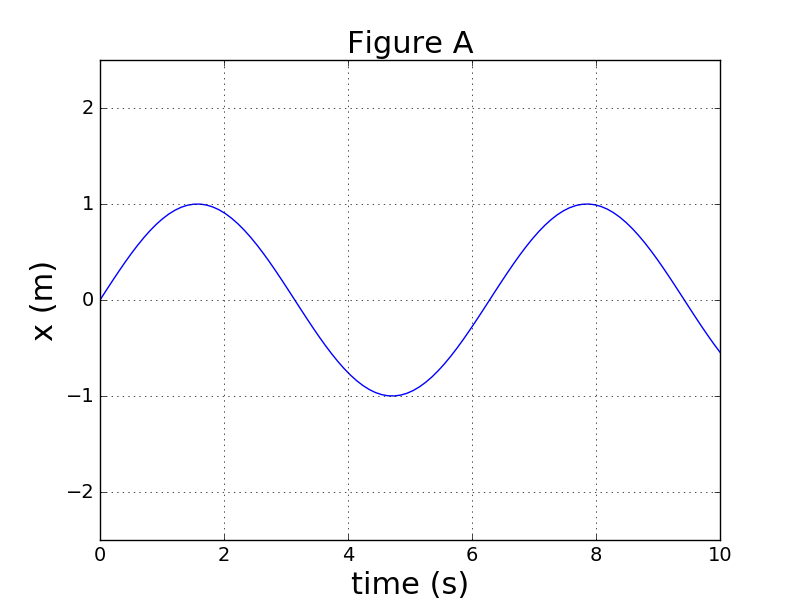
\includegraphics[scale=0.25]{figures/DescribingMotionin1D/XfromAcheckpointFigA.png}
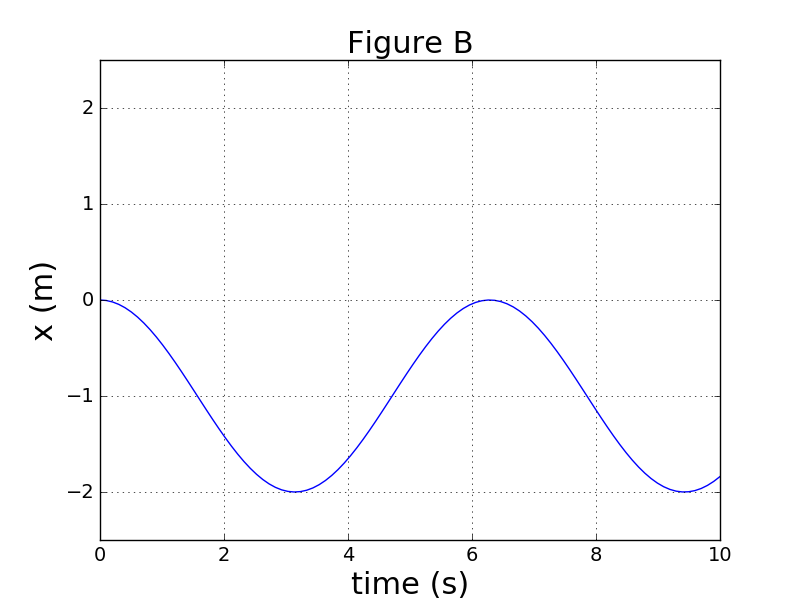
\includegraphics[scale=0.25]{figures/DescribingMotionin1D/XfromAcheckpointFigB.png}
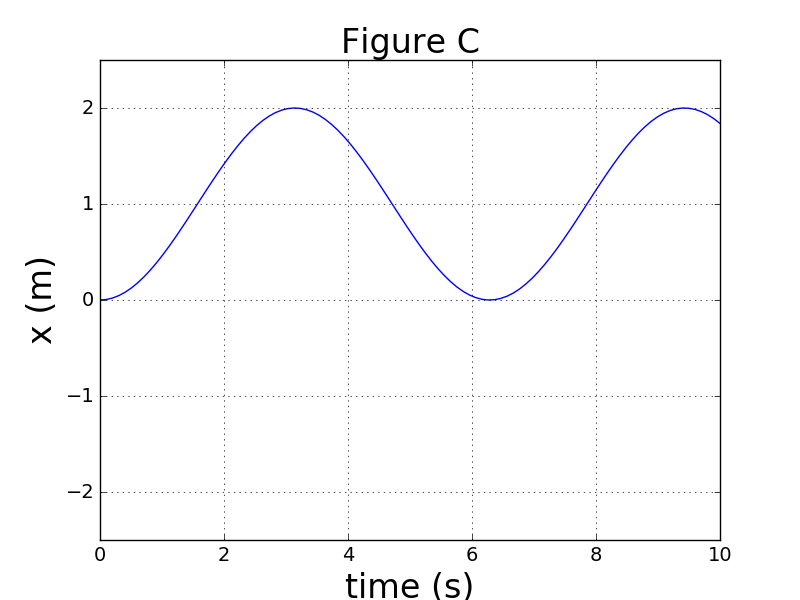
\includegraphics[scale=0.25]{figures/DescribingMotionin1D/XfromAcheckpointFigC.png}
\end{center}
\begin{enumerate}[label=\Alph*)]
\item Figure A
\item Figure B
\item Figure C
\end{enumerate}
\end{checkpointSA}



\section{Relative motion}
In order to describe the motion of an object confined to a straight line, we introduced an axis ($x$) with a specified direction (in which $x$ increases) and an origin (where $x=0$). Sometimes, it can be more convenient to use an axis that is \textit{moving}. For example, consider a person, Alice, moving inside of a train headed for the French town of Nice. The train is moving with a constant speed, $v'^B$ as measured from the ground. Suppose that another person, Brice, describes Alice's position using the function $x^A(t)$ using an x-axis defined inside of the train car ($x=0$ where Brice is sitting, and positive $x$ is in the direction of the train's motion), as depicted in Figure \ref{fig:DescribingMotionIn1D:TrainABC} below. As long as any person is in the train with Brice, they will easily be able to describe Alice's motion using the x-axis that is moving with the train. Suppose that the train goes through the French town of Hossegor, where a surfer, Igor, watches the train go by. If Igor wishes to describe Alice's motion, it is easier for him to use a different axis, say $x'$, that is fixed to the ground and not moving with the train. 
\capfig{0.7\textwidth}{figures/DescribingMotionIn1D/TrainABC.png}{\label{fig:DescribingMotionIn1D:TrainABC}Alice is walking in the train and her position is described by both Brice, who is sitting in the train (using the $x$ axis), and Igor, who is at rest on the ground (using the $x'$ axis).} 

Since Brice already went through the work of determining the function $x^A(t)$ in the \textbf{reference frame} of the train, we wish to determine how to \textit{transform} $x^A(t)$ into the reference frame of the train station, $x'^A(t)$, so that Igor can also describe Alice's motion. In other words, we wish to describe Alice's motion in two different \textit{reference frames}.


A reference frame is simply a choice of coordinates, in this case, a choice of x-axis. Ideally, in physics, we prefer to use \textit{inertial} reference frames, which are reference frames that are either ``at rest'' or that are moving at a constant speed relative to a frame that we consider at rest.
 
 
In principle, if you blocked out all of the windows in the train, it would not be possible for Alice and Brice to determine if the train is moving at constant speed or if it is stopped. Thus, the concept of a ``rest frame'' is itself arbitrary. It is not possible to define a frame of reference that is truly at rest. Even Igor's frame of reference, the train station, is on the planet Earth, which is moving around the Sun with a speed of \SI{108000}{km/h}.


Not only is it impossible to define a frame of reference that is truly at rest, the rules from transforming from one frame to the other depend on the speed between the reference frames. Our common experience is described by what we call ``Galilean Relativity'', but if the speed between trains is very large, close to the speed of light, then we need to use Einstein's Special Theory of Relativity.

Referring to Figure \ref{fig:DescribingMotionIn1D:TrainABC}, we wish to use Brice's description of Alice's motion, $x^A(t)$, and convert it into a description, $x'^A(t)$ that Igor can use in the train station. Since Brice is at rest in the train, the speed of Brice \textit{relative} to Igor is $v'^B(t)$. The first step is for Igor to describe Brice's position, $x'^B(t)$, (that is, the position of Brice's origin). Assume that we choose $t=0$ to be the point in time where the two origins are aligned. Since the train is moving at a constant speed, $v_B$ (as measured by Brice), then the position of Brice's origin as measured from Igor's origin is given by:
\begin{align*}
x'^B(t)=v'^Bt
\end{align*}
Now that Igor can describe the position of the origin of Brice's coordinate system, he can use Brice's description of Alice's motion. Recall that $x^A(t)$ is Brice's measure of Alice's distance from his origin. Similarly, $x'^B(t)$, is Igor's measure of the distance from his origin to Brice's origin. Thus, to obtain Alice's distance from Igor's origin, we simply add the distance, $x'^B(t)$, from Igor's origin to Brice's origin, and then add, $x^A(t)$, the distance from Brice's origin to Alice. Thus:
\begin{align}
\Aboxed{x'^A(t)=x'^B(t)+x^A(t)=v'^Bt+x^A(t)}
\end{align}
which tells us how to obtain the position of object A in the $x'$ reference frame, when $x^A(t)$ is the description the object's position in the $x$ reference frame which is moving with a velocity $v'^B$ relative to the $x'$ reference frame.

Since we know the position of Alice as measured in Igor's frame of reference, we can now easily find her velocity and her acceleration, as measured by Igor. Her velocity as measured by Igor, $v'^A$, is given by the time-derivative of her position measured in Igor's frame of reference:
\begin{align}
v'^A(t)&=\frac{d}{dt}x'^A(t)\\
&=\frac{d}{dt}(v'^Bt+x^A(t))\\
&=v'^B+\frac{d}{dt}x^A(t)\\
&=v'^B+v^A(t)
\end{align}
where $v^A(t)=\frac{d}{dt}x^A(t)$ is Alice's speed as measured by Brice, in the train. That is, the velocity of Alice as measured by Igor is the sum of the velocity of the train relative to the ground and the velocity of Alice relative to the train, which makes sense. If we now determine Alice's acceleration, $a'^A(t)$, as measured by Igor, we find:
\begin{align}
a'^A(t)&=\frac{d}{dt}v'^A(t)\\
&=\frac{d}{dt}(v'^B+v^A)\\
&=0+\frac{d}{dt}v^A(t)\\
&=a^A
\end{align}
where we have explicitly used the fact that the train is moving at constant velocity ($\frac{d}{dt}v'^B=0$). Here we find that both Brice and Igor will measure the same number when referring to Alice's acceleration (if the train is moving at a constant velocity). This is a particularity of ``inertial'' frame of references: accelerations do not depend on the reference frame, as long as the reference frames are moving with a constant velocity relative to each other. As we will see later, forces exerted on an object are directly related to the acceleration experienced by that object. Thus, the forces on an object do not depend on the choice of inertial reference frame. 

\begin{example}{A large boat is sailing North at a speed of $v'^B=\SI{15}{m/s}$ and a restless passenger is walking about on the deck. Chlo\"e, another passenger on the boat, finds that the passenger is walking at a constant speed of $v^A=\SI{3}{m/s}$ towards the South (opposite the direction of the boat's motion). Marcel is watching the boat pass by from the shore. What velocity (magnitude and direction) does Marcel measure for the restless passenger?}
First, we must choose coordinate systems in the boat and on the shore. On the boat, let us define an $x$ axis that is positive in the North direction and has an origin such that the position of the restless passenger was $x^A(t=0)=0$ at time $t=0$. In Chlo\"e's reference frame, the passenger is thus described by:
\begin{align*}
x^A(t)=v^At=(\SI{-3}{m/s})t
\end{align*}
where we note that $v^A$ is negative since the passenger is moving the in negative $x$ direction (the passenger is walking towards the South, but we chose positive $x$ to be in the North direction). On shore, we choose an $x'$ axis that also is positive in the North direction. We can choose the origin such that the origin of the boat's coordinate system was $x'=0$. The origin of the boat's coordinate system as measured by Marcel (on shore) is thus:
\begin{align*}
x'^B(t)=v'^Bt=(\SI{15}{m/s})t
\end{align*}
The position of the passenger, $x'^A(t)$, as measured by Marcel, is then given by adding the position of the boat's origin and the position of the passenger as measured from the boat's origin:
\begin{align*}
x'^A(t) &= x'^B(t)+x^A(t)\\
&= v'^Bt + v^At \\
&= (v'^B+v^A)t\\
&= ((\SI{15}{m/s})+(\SI{-3}{m/s}))t\\
&= (\SI{12}{m/s})t
\end{align*}
To find the velocity of the passenger as measured by Marcel, we take the time derivative:
\begin{align*}
v'^A &= \frac{d}{dt}x'^A(t)\\
&= \frac{d}{dt} \left((v'^B+v^A)t\right)\\
&=(v'^B+v^A)\\
&=((\SI{15}{m/s})+(\SI{-3}{m/s}))\\
&=\SI{12}{m/s}
\end{align*}
Since this is a positive number, Marcel still sees the passenger moving in the North direction (the direction of his positive $x'$ axis), but with a speed of \SI{12}{m/s}, which is less than that of the boat. On the boat, the passenger appears to be walking towards the South, but the net motion of the passenger relative to the ground is still in the North direction, as their speed is less than that of the boat.
\end{example}


\newpage
\section{Summary}
\vspace{1cm}
\begin{chapterSummary}
\item To describe motion in one dimension, we must define an axis with:
\begin{enumerate}
\item An origin (where $x=0$)
\item A direction (the direction in which $x$ increases).
\end{enumerate}
\item We describe the position of an object with a function $x(t)$ that \textit{depends} on time.
\item The rate of change of position is called ``velocity'' and is a function given by the time-derivative of position.
\item The rate of change of velocity is called ``acceleration'' and is a function given by the time-derivative of velocity.
\item Given a function for acceleration, $a_x(t)$, one can use its anti-derivative to determine velocity.
\item Given a function for velocity, $v_x(t)$, one can use its anti-derivative to determine position.
\item An inertial frame of reference is one that is moving with a constant velocity.
\item It is impossible to define a frame of reference that is truly ``at rest'', so we consider inertial frames of reference only relative to other frames of reference that we also consider to be inertial.
\item If an object has a position $x^A(t)$ in a given inertial frame of reference, $x$, that is moving with a velocity $v'^B$ compared to a different inertial frame of reference, $x'$, then the position of the object in the $x'$ frame of reference is given by $x'(t)=v'^B+x^A(t)$.
\end{chapterSummary}
\subsection{Important equations}
If the position of an object is described by a function $x(t)$, then, its velocity, $v_x(t)$, and acceleration, $a_x(t)$, are given by:
\begin{align*}
v_x(t)&=\lim_{\Delta t\to 0}\frac{\Delta x}{\Delta t}=\frac{dx}{dt}\\
a_x(t)&=\lim_{\Delta t\to 0}\frac{\Delta v}{\Delta t}=\frac{dv_x}{dt}\\
\end{align*}
Conversely, given the acceleration, $a_x(t)$, on can find the velocity and position:
\begin{align*}
v_x(t)&=\int a_x(t)dt\\
x(t)&=\int v_x(t)dt\\
\end{align*}
With a constant acceleration, $a_x(t)=a_x$, if the object had velocity $v_{0x}$ and position $x_0$ at $t=0$:
\begin{align*}
v_x(t)&=v_{0x}t+a_xt\\
x(t)&=x_0+v_{0x}t+\frac{1}{2}a_xt^2
\end{align*}
If an object has position $x^A$ as measured in a frame of reference $x$ that is moving at constant speed $v'^B$ as measured in a second frame of reference $x'$, then in the $x'$ reference frame, the kinematic quantities for the object are obtained by the Galilean transformation:
\begin{align*}
x'^A(t) &= v'^Bt + x^A(t)\\
v'^A(t) &=v'^B+v^A(t)\\
a'^A(t) &= a(t)
\end{align*}

\section{Problems}

\begin{problemParts}{Rob is riding is bike at a speed of $\SI{8}{m/s}$. He passes by a velociraptor, as one often does, who is eating by the side of the road. The velociraptor begins chasing him. The velociraptor accelerates from rest at a rate of $\SI{4}{m/s^2}$.} 
\item Assuming it takes 3 seconds for the velociraptor to react, how long does it take from the moment Rob passes by for the velicoraptor to catch up to him? 
\item If there is a safe place 70 metres from where Rob passes the velociraptor, will Rob make it there in time to escape being eaten?  
\end{problemParts}

\textbf{Solution:}\\
We start by choosing our coordinate system. The solution is simplest if the $x$ axis is positive in the direction of motion and has an origin at the point where Rob passes the velociraptor. We set $t=0$ to be the moment the velociraptor starts running.\\

\capfig{\textwidth}{figures/DescribingMotionIn1D/VelociraptorQuestion.png}{\label{fig:VelociraptorProblem1D} Rob is being chased by a velociraptor. At $t=0$, Rob is a distance $x_{0R}$ from the velociraptor. Safety is $\SI{70}{m}$ away from the origin.}

Since we are dealing with constant accelerations, we can use the equation:
\begin{align*}
x(t)&=x_0+v_{0x}t+\frac{1}{2}a_xt^2
\end{align*}
We can use a table to take stock of our known values and variables:
\begin{table}[h!]
\centering
\label{KnownsUnknownsSampleProb1D}
\begin{tabular}{|c|c|}
\hline
\textbf{Rob}          & \textbf{Velociraptor}  \\ \hline
$x_{0R} = ?$          & $x_{0V} = \SI{0}{m}$   \\
$v_R = \SI{8}{m/s}$   & $v_{0V} = \SI{0}{m/s}$ \\
$a_R = \SI{0}{m/s^2}$ & $a_V = \SI{4}{m/s^2}$  \\
$t$                   & $t$                    \\
$x_R$                 & $x_V$                 
\end{tabular}
\end{table}

The value of $x_{0R}$ is unknown but can be easily solved for. We defined $t=0$ as the moment the velociraptor starts running. It takes 3 seconds for the velociraptor to react, so at $t=0$, Rob has moved $(\SI{8}{m/s})\times (\SI{3}{s}) = \SI{24}{m}$.\\

Next, we can write out our equations as,
\begin{align*}
x_R&=x_{0R}+v_{R}t\\
x_V&=\frac{1}{2}a_Vt^2
\end{align*}
 
Now what do we mean by ``catch up"? It means that Rob and the velociraptor are in the same place at the same time. So, we are interested in the value of $t$ when $x_R=x_V$. Setting the above equations equal to one another gives
\begin{align*}
x_{0R}+v_{R}t&=\frac{1}{2}a_Vt^2 
\end{align*}
that we can rearrange to get this quadratic:
\begin{align*}
0&=\frac{1}{2}a_Vt^2-v_{R}t-x_{0R} 
\end{align*}

By solving the quadratic, we find that $t=\SI{6}{s}$. This doesn't quite give us the answer we want. We want to know how long it takes the velociraptor to catch up \textit{from the moment Rob passes by}, so we have to add on the $\SI{3}{s}$ reaction time, giving a total time of $\SI{9}{s}$.\\

We can use this solution to figure out whether Rob makes it to safety. In 9 seconds, Rob travels a distance of $(\SI{8}{m/s})\times (\SI{9}{s}) = \SI{72}{m}$. The shelter is only $\SI{70}{m}$ away, so Rob gets to safety in time!


\begin{problem} Figure \ref{fig:AccelerationProblem1D} shows a graph of the acceleration, $a(t)$, of a particle moving in one dimension. Draw the corresponding velocity and position graphs. Assume that $v(0)=x(0)=0$. 
\end{problem}
\capfig{0.6\textwidth}{figures/DescribingMotionIn1D/AccelerationProblem.jpg}{\label{fig:AccelerationProblem1D}A graph of acceleration as a function of time. The scale and units are arbitrary.}
\textbf{Solution:}
\begin{center}
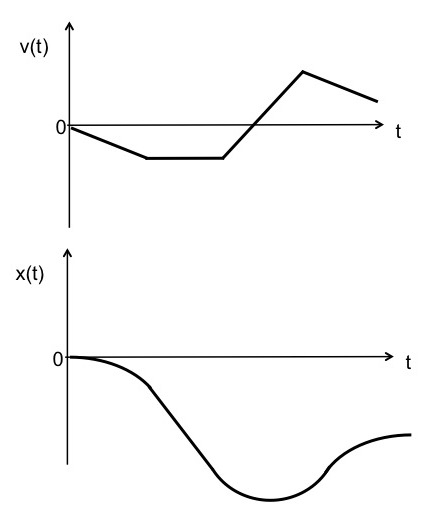
\includegraphics[scale=0.6]{figures/DescribingMotionIn1D/VelocityPositionProblem.jpg}{\label{fig:VelocityPositionProblem1D}}
\end{center}
Solutions may vary, however there are a few key features that must be present.\\
For the graph of $v(t)$:
\begin{itemize}
\item Velocity is zero at $t=0$.
\item When acceleration is negative, the velocity is (negative slope). It follows that when the acceleration is positive, the velocity is increasing. 
\item When the acceleration is zero, the velocity should be a flat line
\end{itemize}
For the graph of $x(t)$:
\begin{itemize}
\item Position is zero at $x=0$
\item When velocity is negative, $x(t)$ is decreasing. When velocity is positive, $x(t)$ is increasing
\item Take note of the turning points on the graph of $x(t)$.The particle turns around (the position goes from increasing or decreasing, or from decreasing to increasing) when the velocity changes sign. 
\item When the velocity and acceleration are in the same direction, the slope of $x(t)$ increases in magnitude. When the acceleration and velocity are in opposite directions, the slope of $x(t)$ decreases in magnitude. 
\end{itemize}

\begin{reflectresearch}\\
Look up the depth of a competition diving pool. What is the relationship between the height of the diving platform and the minimum pool depth? Why? If the designers of the pool assumed that every diver drops straight down off the diving board, would the pool still be safe for divers that jump up first?
\end{reflectresearch}
